\documentclass[11pt,a4paper]{article}
\usepackage[utf8]{inputenc}
\usepackage[english]{babel}
\usepackage{fontspec}
\usepackage{xunicode}
\usepackage{xltxtra}
\usepackage{polyglossia}
\usepackage{amsmath}
\usepackage{amsfonts}
\usepackage{amssymb}
\usepackage{graphicx}
\usepackage[left=2cm,right=2cm,top=2cm,bottom=2cm]{geometry}
\usepackage{afterpage}
\usepackage{xcolor}
\usepackage{pagecolor}
\usepackage{mathtools}
%\usepackage{fancyhdr}
\usepackage{hyperref}
\usepackage{blindtext}
\usepackage{mahjong}
\usepackage{amsthm}
\usepackage{chngcntr}
\usepackage{tikz}
\usepackage{bbold}
\usepackage{pdfpages}

\usepackage{stmaryrd}
\let\stmaryrdLightning\lightning

\author{Zehao Gao}

\begin{document}

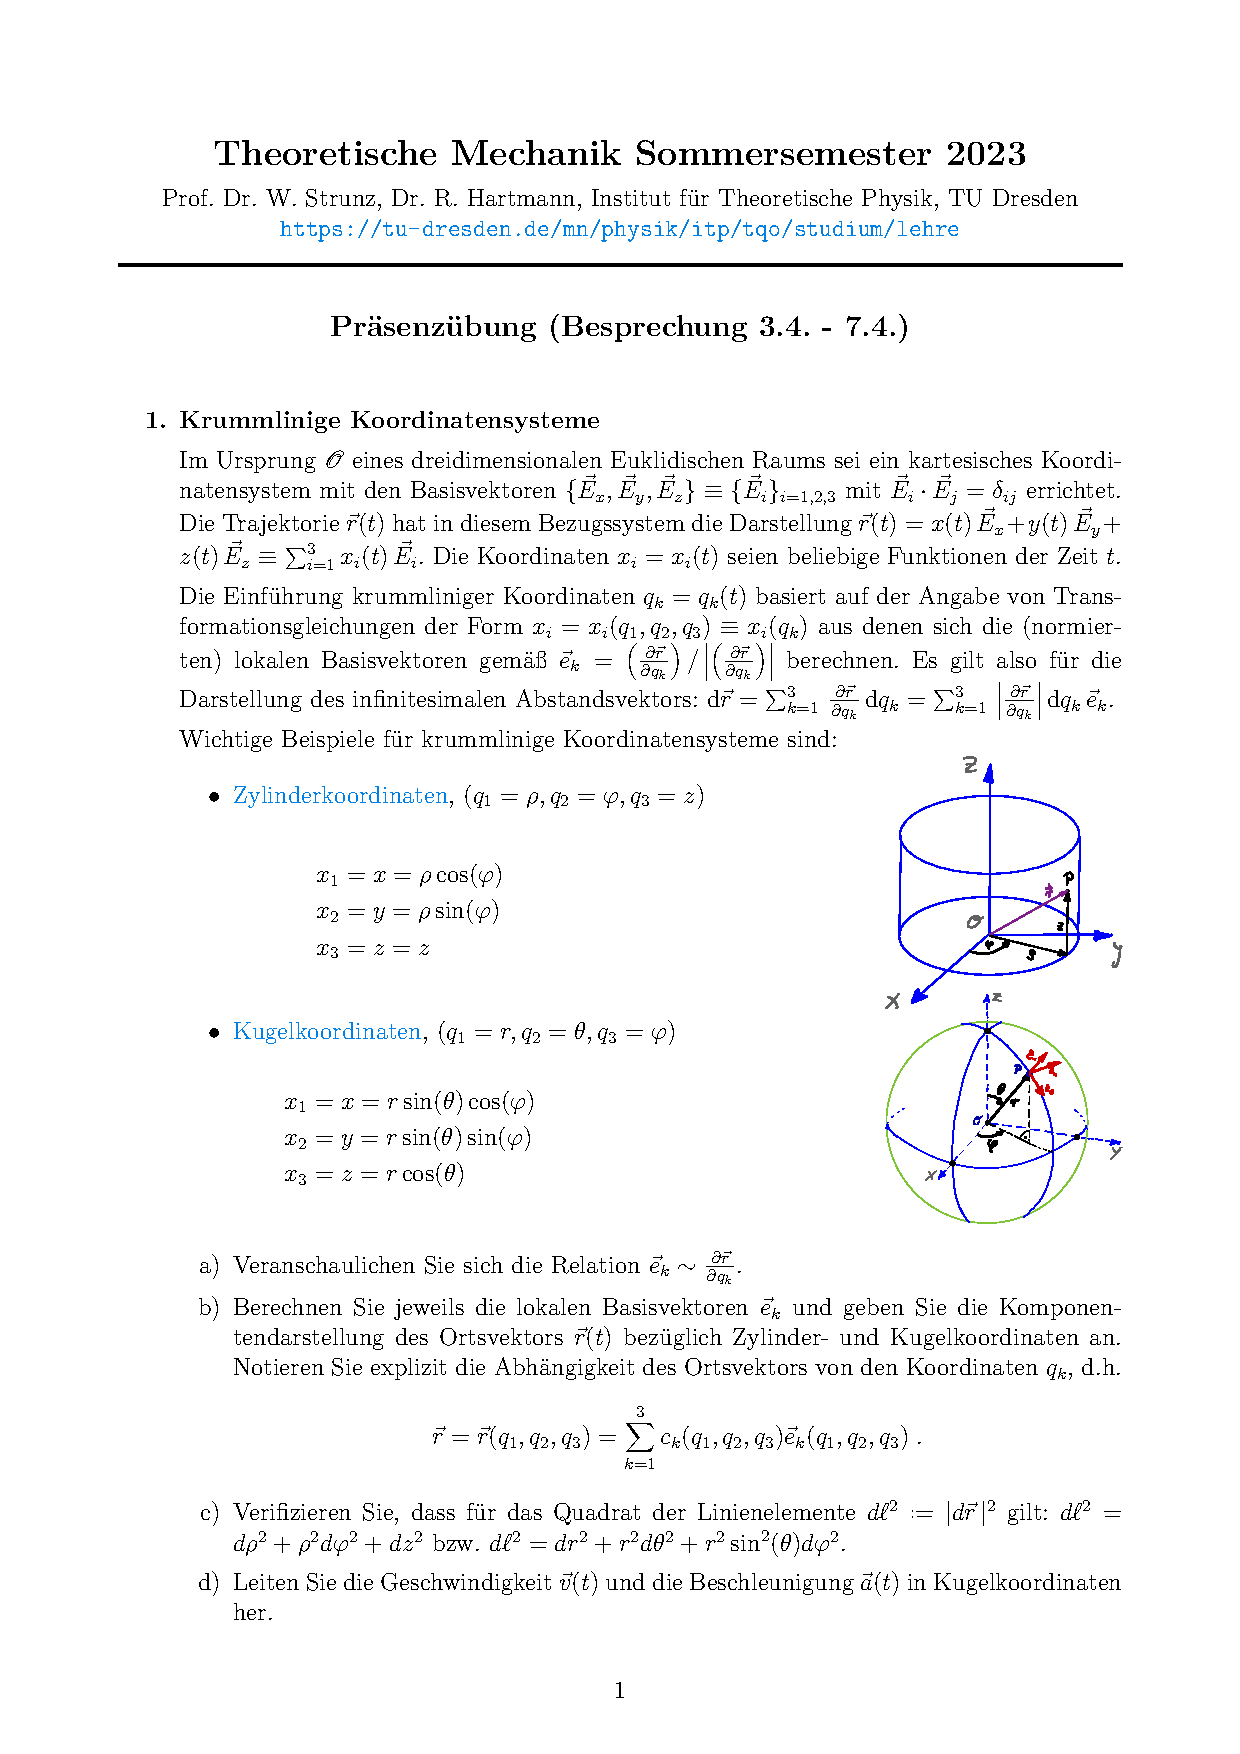
\includepdf[pages=-]{TM_2023_00.pdf}

\section*{Homework 0 solutions}

\paragraph{Question 1}

\begin{enumerate}
\item[(a)]

\begin{equation}
\hat{q}_k=\frac{1}{|\frac{\partial\vec{r}}{\partial q_k}|}\frac{\partial\vec{r}}{\partial q_k}
\end{equation}

The relation between two curvilinear coordinates and Cartesian coordinates are given by
\begin{align*}
&\textrm{cylindrical coordinates}\ (\rho,\varphi,z)\\
&x=\rho\cos(\varphi)\\
&y=\rho\sin(\varphi)\\
&z=z
\end{align*}
\begin{align*}
&\textrm{spherical coordinates}\ (r,\vartheta,\varphi)\\
&x=r\sin(\vartheta)\cos(\varphi)\\
&y=r\sin(\vartheta)\sin(\varphi)\\
&z=r\cos(\vartheta)
\end{align*}

We do a transformation using equation (1) to spherical coordinates:
\begin{equation*}
\vec{r}=
\begin{bmatrix}
x \\
y \\
z
\end{bmatrix}
=
\begin{bmatrix}
r\sin(\vartheta)\cos(\varphi) \\
r\sin(\vartheta)\sin(\varphi) \\
r\cos(\vartheta)
\end{bmatrix}
\end{equation*}
\begin{equation*}
\frac{\partial\vec{r}}{\partial r}
=
\begin{bmatrix}
\sin(\vartheta)\cos(\varphi) \\
\sin(\vartheta)\sin(\varphi) \\
\cos(\vartheta)
\end{bmatrix},\ 
\frac{\partial\vec{r}}{\partial \vartheta}
=
\begin{bmatrix}
r\cos(\vartheta)\cos(\varphi) \\
r\cos(\vartheta)\sin(\varphi) \\
-r\sin(\vartheta)
\end{bmatrix},\ 
\frac{\partial\vec{r}}{\partial \varphi}
=
\begin{bmatrix}
-r\sin(\vartheta)\sin(\varphi) \\
r\sin(\vartheta)\cos(\varphi) \\
0
\end{bmatrix}
\end{equation*}

with
\begin{align*}
\bigg|\frac{\partial\vec{r}}{\partial r}\bigg|&=\sqrt{\sin^2(\vartheta)\cos^2(\varphi)+\sin^2(\vartheta)\sin^2(\varphi)+\cos^2(\vartheta)}=1 \\
\bigg|\frac{\partial\vec{r}}{\partial \vartheta}\bigg|&=\sqrt{r\cos^2(\vartheta)\cos^2(\varphi)+r^2\cos^2(\vartheta)\sin^2(\varphi)+r^2\sin^2(\vartheta)}=r \\
\bigg|\frac{\partial\vec{r}}{\partial \varphi}\bigg|&=\sqrt{r^2\sin^2(\vartheta)\sin^2(\varphi)+r^2\sin^2(\vartheta)\cos^2(\varphi)}=r\sin(\vartheta)
\end{align*}

we get the unit vectors:
\begin{equation}
\hat{r}=
\begin{bmatrix}
\sin(\vartheta)\cos(\varphi) \\
\sin(\vartheta)\sin(\varphi) \\
\cos(\vartheta)
\end{bmatrix},\ 
\hat{\vartheta}=
\begin{bmatrix}
\cos(\vartheta)\cos(\varphi) \\
\cos(\vartheta)\sin(\varphi) \\
-\sin(\vartheta)
\end{bmatrix},\ 
\hat{\varphi}=
\begin{bmatrix}
-\sin(\varphi) \\
\cos(\varphi) \\
0
\end{bmatrix}
\end{equation}

with transformation matrix:
\begin{align}
\begin{bmatrix}
\hat{r} \\
\hat{\vartheta} \\
\hat{\varphi}
\end{bmatrix}
&=
\begin{bmatrix}
\sin(\vartheta)\cos(\varphi) & \sin(\vartheta)\sin(\varphi) & \cos(\vartheta) \\
\cos(\vartheta)\cos(\varphi) & \cos(\vartheta)\sin(\varphi) & -\sin(\vartheta) \\
-\sin(\varphi) & \cos(\varphi) & 0
\end{bmatrix}
\begin{bmatrix}
\hat{x} \\
\hat{y} \\
\hat{z}
\end{bmatrix} \\
\Rightarrow
\begin{bmatrix}
\hat{x} \\
\hat{y} \\
\hat{z}
\end{bmatrix}
&=
\begin{bmatrix}
\sin(\vartheta)\cos(\varphi) & \cos(\vartheta)\cos(\varphi) & -\sin(\varphi) \\
\sin(\vartheta)\sin(\varphi) & \cos(\vartheta)\sin(\varphi) & \cos(\varphi) \\
\cos(\vartheta) & -\sin(\vartheta) & 0
\end{bmatrix}
\begin{bmatrix}
\hat{r} \\
\hat{\vartheta} \\
\hat{\varphi}
\end{bmatrix}
\end{align}

\newpage

We now verify the orthogonality of our new unit vectors using cross product:
\begin{align*}
\hat{r}\times\hat{\vartheta}
&=
\begin{bmatrix}
\sin(\vartheta)\sin(\varphi)(-\sin(\vartheta))-\cos(\vartheta)\cos(\vartheta)\sin(\varphi) \\
\cos(\vartheta)\cos(\vartheta)\cos(\varphi)-\sin(\vartheta)\cos(\varphi)(-\sin(\vartheta)) \\
\sin(\vartheta)\cos(\varphi)\cos(\vartheta)\sin(\varphi)-\sin(\vartheta)\sin(\varphi)\cos(\vartheta)\cos(\varphi)
\end{bmatrix}\\
&=
\begin{bmatrix}
-(\sin^2(\vartheta)\sin(\varphi)+\cos^2(\vartheta)\sin(\varphi)) \\
\cos^2(\vartheta)\cos(\varphi)+\sin^2(\vartheta)\cos(\varphi) \\
\sin(\vartheta)\cos(\varphi)\cos(\vartheta)\sin(\varphi)-\sin(\vartheta)\sin(\varphi)\cos(\vartheta)\cos(\varphi)
\end{bmatrix}
=
\begin{bmatrix}
-\sin(\varphi) \\
\cos(\varphi) \\
0
\end{bmatrix}
=\hat{\varphi}
\end{align*}

correct, but I wanna do a double check:
\begin{align*}
\hat{\vartheta}\times\hat{\varphi}
=
\begin{bmatrix}
\cos(\vartheta)\sin(\varphi)0-(-\sin(\vartheta))\cos(\varphi) \\
(-\sin(\vartheta))(-\sin(\varphi))-\cos(\vartheta)\cos(\varphi)0 \\
\cos(\vartheta)\cos(\varphi)\cos(\varphi)-\cos(\vartheta)\sin(\varphi)(-\sin(\varphi))
\end{bmatrix}
=
\begin{bmatrix}
\sin(\vartheta)\cos(\varphi) \\
\sin(\vartheta)\sin(\varphi) \\
\cos(\vartheta)
\end{bmatrix}
=\hat{r}
\end{align*}

%definitely correct.

Now we do the same transformation to cylindrical coordinates:
\begin{equation*}
\vec{r}=
\begin{bmatrix}
\rho\cos(\varphi) \\
\rho\sin(\varphi) \\
z
\end{bmatrix}
\end{equation*}
\begin{equation*}
\frac{\partial\vec{r}}{\partial\rho}=
\begin{bmatrix}
\cos(\varphi) \\
\sin(\varphi) \\
0
\end{bmatrix},\ 
\frac{\partial\vec{r}}{\partial\varphi}=
\begin{bmatrix}
-\rho\sin(\varphi) \\
\rho\cos(\varphi) \\
0
\end{bmatrix},\ 
\frac{\partial\vec{r}}{\partial z}=
\begin{bmatrix}
0 \\
0 \\
1
\end{bmatrix}
\end{equation*}

with
\begin{align*}
\bigg|\frac{\partial\vec{r}}{\partial\rho}\bigg|&=\sqrt{\cos^2(\varphi)+\sin^2(\varphi)}=1 \\
\bigg|\frac{\partial\vec{r}}{\partial\varphi}\bigg|&=\sqrt{\rho^2\sin^2(\varphi)+\rho^2\cos^2(\varphi)}=\rho \\
\bigg|\frac{\partial\vec{r}}{\partial z}\bigg|&=1
\end{align*}

therefore:
\begin{equation}
\hat{\rho}=
\begin{bmatrix}
\cos(\varphi) \\
\sin(\varphi) \\
0
\end{bmatrix},\
\hat{\varphi}=
\begin{bmatrix}
-\sin(\varphi) \\
\cos(\varphi) \\
0
\end{bmatrix},\
\hat{z}=
\begin{bmatrix}
0 \\
0 \\
1
\end{bmatrix}
\end{equation}

with transformation matrix:
\begin{align}
\begin{bmatrix}
\hat{\rho} \\
\hat{\varphi} \\
z
\end{bmatrix}
&=
\begin{bmatrix}
\cos(\varphi) & \sin(\varphi) & 0 \\
-\sin(\varphi) & \cos(\varphi) & 0 \\
0 & 0 & 1
\end{bmatrix}
\begin{bmatrix}
\hat{x} \\
\hat{y} \\
\hat{z}
\end{bmatrix}
\\
\Rightarrow
\begin{bmatrix}
\hat{x} \\
\hat{y} \\
\hat{z}
\end{bmatrix}
&=
\begin{bmatrix}
\cos(\varphi) & -\sin(\varphi) & 0 \\
\sin(\varphi) & \cos(\varphi) & 0 \\
0 & 0 & 1
\end{bmatrix}
\begin{bmatrix}
\hat{\rho} \\
\hat{\varphi} \\
\hat{z}
\end{bmatrix}
\end{align}

\newpage

\item[(b)]

The position vector $\vec{r}$ in combination of basis vectors from cartesian coordinates and factors of curvilinear coordinates is given by
\begin{align}
(sperical)\ \vec{r}&=r\sin(\vartheta)\cos(\varphi)\hat{x}+r\sin(\vartheta)\sin(\varphi)\hat{y}+r\cos(\vartheta)\hat{z}\\
(cylindrical)\ \vec{r}&=\rho\cos(\varphi)\hat{x}+\rho\sin(\varphi)\hat{y}+z\hat{z}
\end{align}

our goal is to obtain an expression of position vector, such that it is explicitly expressed by curvilinear coordinates, like in the following equation:
\begin{align*}
\vec{r}=\vec{r}(q_1,q_2,q_3)=\sum_{k=1}^3c_k(q_1,q_2,q_3)\hat{q}_k(q_1,q_2,q_3)
\end{align*}

Now we replace unit vectors of cartesian coordinates with which from curvilinear coordinates using transformation matrices.

For spherical coordinates, we use equation (4):

\begin{equation*}
\begin{bmatrix}
\hat{x} \\
\hat{y} \\
\hat{z}
\end{bmatrix}
=
\begin{bmatrix}
\sin(\vartheta)\cos(\varphi) & \cos(\vartheta)\cos(\varphi) & -\sin(\varphi) \\
\sin(\vartheta)\sin(\varphi) & \cos(\vartheta)\sin(\varphi) & \cos(\varphi) \\
\cos(\vartheta) & -\sin(\vartheta) & 0
\end{bmatrix}
\begin{bmatrix}
\hat{r} \\
\hat{\vartheta} \\
\hat{\varphi}
\end{bmatrix}
\end{equation*}

we insert position vector form (8),
\begin{align*}
&
\begin{bmatrix}
r\sin(\vartheta)\cos(\varphi) & & \\
& r\sin(\vartheta)\sin(\varphi) & \\
& & r\cos(\vartheta)
\end{bmatrix}
\begin{bmatrix}
\hat{x} \\
\hat{y} \\
\hat{z}
\end{bmatrix}\\
=&
\begin{bmatrix}
r\sin(\vartheta)\cos(\varphi) & & \\
& r\sin(\vartheta)\sin(\varphi) & \\
& & r\cos(\vartheta)
\end{bmatrix}
\begin{bmatrix}
\sin(\vartheta)\cos(\varphi) & \cos(\vartheta)\cos(\varphi) & -\sin(\varphi) \\
\sin(\vartheta)\sin(\varphi) & \cos(\vartheta)\sin(\varphi) & \cos(\varphi) \\
\cos(\vartheta) & -\sin(\vartheta) & 0
\end{bmatrix}
\begin{bmatrix}
\hat{r} \\
\hat{\vartheta} \\
\hat{\varphi}
\end{bmatrix}\\
=&
\begin{bmatrix}
r\sin^2(\vartheta)\cos^2(\varphi) & r\sin(\vartheta)\cos(\vartheta)\cos^2(\varphi) & -r\sin(\vartheta)\cos(\varphi)\sin(\varphi) \\
r\sin^2(\vartheta)\sin^2(\varphi) & r\sin(\vartheta)\cos(\vartheta)\sin^2(\varphi) & r\sin(\vartheta)\sin(\varphi)\cos(\varphi) \\
r\cos^2(\vartheta) & -r\cos(\vartheta)\sin(\vartheta) & 0
\end{bmatrix}
\begin{bmatrix}
\hat{r} \\
\hat{\vartheta} \\
\hat{\varphi}
\end{bmatrix}\\
=&
\begin{bmatrix}
r\sin^2(\vartheta)\cos^2(\varphi)\hat{r}+r\sin(\vartheta)\cos(\vartheta)\cos^2(\varphi)\hat{\vartheta}-r\sin(\vartheta)\cos(\varphi)\sin(\varphi)\hat{\varphi} \\
r\sin^2(\vartheta)\sin^2(\varphi)\hat{r}+r\sin(\vartheta)\cos(\vartheta)\sin^2(\varphi)\hat{\vartheta}+r\sin(\vartheta)\sin(\varphi)\cos(\varphi)\hat{\varphi} \\
r\cos^2(\vartheta)\hat{r}-r\cos(\vartheta)\sin(\vartheta)\hat{\vartheta}
\end{bmatrix}\\
\begin{split}
=&
(r\sin^2(\vartheta)\cos^2(\varphi)+r\sin^2(\vartheta)\sin^2(\varphi)+r\cos^2(\vartheta))\hat{r}\\
&+(r\sin(\vartheta)\cos(\vartheta)\cos^2(\varphi)+r\sin(\vartheta)\cos(\vartheta)\sin^2(\varphi)-r\cos(\vartheta)\sin(\vartheta))\hat{\vartheta}\\
&+(-r\sin(\vartheta)\cos(\varphi)\sin(\varphi)+r\sin(\vartheta)\sin(\varphi))\cos(\varphi)\hat{\varphi}
\end{split}\\
=&
r\hat{r}
\end{align*}

\newpage

And for cylindrical coordinates:
\begin{align*}
\begin{bmatrix}
\rho\cos(\varphi) & & \\
& \rho\sin(\varphi) & \\
& & z
\end{bmatrix}
\begin{bmatrix}
\hat{x} \\
\hat{y} \\
\hat{z}
\end{bmatrix}
=&
\begin{bmatrix}
\rho\cos(\varphi) & & \\
& \rho\sin(\varphi) & \\
& & z
\end{bmatrix}
\begin{bmatrix}
\cos(\varphi) & -\sin(\varphi) & 0 \\
\sin(\varphi) & \cos(\varphi) & 0 \\
0 & 0 & 1
\end{bmatrix}
\begin{bmatrix}
\hat{\rho} \\
\hat{\varphi} \\
\hat{z}
\end{bmatrix}\\
=&
\begin{bmatrix}
\rho\cos^2(\varphi) & -\rho\sin(\varphi)\cos(\varphi) & 0 \\
\rho\sin^2(\varphi) & \rho\sin(\varphi)\cos(\varphi) & 0 \\
0 & 0 & z
\end{bmatrix}
\begin{bmatrix}
\hat{\rho} \\
\hat{\varphi} \\
\hat{z}
\end{bmatrix}\\
=&
\begin{bmatrix}
\rho\cos^2(\varphi)\hat{\rho}-\rho\sin(\varphi)\cos(\varphi)\hat{\varphi} \\
\rho\sin^2(\varphi)\hat{\rho}+\rho\sin(\varphi)\cos(\varphi)\hat{\varphi} \\
z\hat{z}
\end{bmatrix}\\
=&
(\rho\cos^2(\varphi)+\rho\sin^2(\varphi))\hat{\rho}+(-\rho\sin(\varphi)\cos(\varphi)+\rho\sin(\varphi)\cos(\varphi))\hat{\varphi}+z\hat{z}\\
=&\rho\hat{\rho}+z\hat{z}
\end{align*}

\newpage

\item[(c)]

The (square of) line element is given by
\begin{align*}
dl:=|d\vec{r}|^2
\end{align*}

with $d\vec{r}=\frac{\partial\vec{r}}{\partial q_1}dq_1+\frac{\partial\vec{r}}{\partial q_2}dq_2+\frac{\partial\vec{r}}{\partial q_3}dq_3$

In spherical coordinates, it is
\begin{align*}
d\vec{r}
&=\frac{\partial\vec{r}}{\partial r}dr+\frac{\partial\vec{r}}{\partial \vartheta}d\vartheta+\frac{\partial\vec{r}}{\partial \varphi}d\varphi \\
&=
\begin{bmatrix}
\sin(\vartheta)\cos(\varphi) \\
\sin(\vartheta)\sin(\varphi) \\
\cos(\vartheta)
\end{bmatrix}
dr
+
\begin{bmatrix}
r\cos(\vartheta)\cos(\varphi) \\
r\cos(\vartheta)\sin(\varphi) \\
-r\sin(\vartheta)
\end{bmatrix}
d\vartheta
+
\begin{bmatrix}
-r\sin(\vartheta)\sin(\varphi) \\
r\sin(\vartheta)\cos(\varphi) \\
0
\end{bmatrix}
d\varphi
\end{align*}

therefore,
\begin{align*}
|d\vec{r}|^2
&=
\begin{bmatrix}
\sin(\vartheta)^2\cos(\varphi)^2 \\
\sin(\vartheta)^2\sin(\varphi)^2 \\
\cos(\vartheta)^2
\end{bmatrix}
dr^2
+
\begin{bmatrix}
r^2\cos(\vartheta)^2\cos(\varphi)^2 \\
r^2\cos(\vartheta)^2\sin(\varphi)^2 \\
r^2\sin(\vartheta)^2
\end{bmatrix}
d\vartheta^2
+
\begin{bmatrix}
r^2\sin(\vartheta)^2\sin(\varphi)^2 \\
r^2\sin(\vartheta)^2\cos(\varphi)^2 \\
0
\end{bmatrix}
d\varphi^2 \\
&=
dr^2+r^2d\vartheta^2+r^2\sin^2(\theta)d\varphi^2
\end{align*}

In cylindrical coordinates, it is
\begin{align*}
d\vec{r}
&=\frac{\partial\vec{\rho}}{\partial \rho}dr+\frac{\partial\vec{r}}{\partial \varphi}d\varphi+\frac{\partial\vec{r}}{\partial z}dz \\
&=
\begin{bmatrix}
\cos(\varphi) \\
\sin(\varphi) \\
0
\end{bmatrix}
dr
+
\begin{bmatrix}
-\rho\sin(\varphi) \\
\rho\cos(\varphi) \\
0
\end{bmatrix}
d\vartheta
+
\begin{bmatrix}
0 \\
0 \\
1
\end{bmatrix}
d\varphi
\end{align*}

therefore
\begin{align*}
|d\vec{r}|^2
&=
\begin{bmatrix}
\cos^2(\varphi) \\
\sin^2(\varphi) \\
0
\end{bmatrix}
d\rho^2
+
\begin{bmatrix}
\rho^2\sin^2(\varphi) \\
\rho^2\cos^2(\varphi) \\
0
\end{bmatrix}
d\varphi^2
+
\begin{bmatrix}
0 \\
0 \\
1
\end{bmatrix}
dz^2 \\
&=d\rho^2+\rho^2d\varphi^2+dz^2
\end{align*}

\newpage

\item[(d)]

The position vector in spherical coordinates is
\begin{align*}
\vec{r}=r\hat{r}
\end{align*}

the speed $\vec{v}(t)$ is the derivative of position vector $\vec{r}$ with respect to time $t$
\begin{align*}
\vec{v}(t)=\dot{\vec{r}}
&=\frac{dr}{dt}\hat{r}+r\frac{d\hat{r}}{dt} \\
&=
\dot{r}(t)
\begin{bmatrix}
\sin(\vartheta(t))\cos(\varphi(t)) \\
\sin(\vartheta(t))\sin(\varphi(t)) \\
\cos(\vartheta(t))
\end{bmatrix}
+
r(t)
\underset{\mahjong{6z}}{\underbrace{
\frac{d}{dt}
\begin{bmatrix}
\sin(\vartheta(t))\cos(\varphi(t)) \\
\sin(\vartheta(t))\sin(\varphi(t)) \\
\cos(\vartheta(t))
\end{bmatrix}
}} \\
\end{align*}

with
\begin{align*}
\mahjong{6z}
&=
\begin{bmatrix}
\dot{\vartheta}(t)\cos(\vartheta(t))\cos(\varphi(t))-\sin(\vartheta(t))\dot{\varphi}(t)\sin(\varphi(t)) \\
\dot{\vartheta}(t)\cos(\vartheta(t))\sin(\varphi(t))+\sin(\vartheta(t))\dot{\varphi}(t)\cos(\varphi(t)) \\
-\dot{\vartheta}(t)\sin(\vartheta(t)) \\
\end{bmatrix} \\
\end{align*}

therefore
\begin{align}
\vec{v}(t)=
\dot{r}(t)
\underset{\hat{r}(t)}{\underbrace{
\begin{bmatrix}
\sin(\vartheta(t))\cos(\varphi(t)) \\
\sin(\vartheta(t))\sin(\varphi(t)) \\
\cos(\vartheta(t))
\end{bmatrix}
}}
+
r(t)
\underset{\dot{\hat{r}}(t)}{\underbrace{
\begin{bmatrix}
\dot{\vartheta}(t)\cos(\vartheta(t))\cos(\varphi(t))-\sin(\vartheta(t))\dot{\varphi}(t)\sin(\varphi(t)) \\
\dot{\vartheta}(t)\cos(\vartheta(t))\sin(\varphi(t))+\sin(\vartheta(t))\dot{\varphi}(t)\cos(\varphi(t)) \\
-\dot{\vartheta}(t)\sin(\vartheta(t)) \\
\end{bmatrix}
}}
\end{align}

the acceleration $a$ is given by
\begin{align}
\vec{a}(t)=\dot{\vec{v}}(t)=\ddot{\vec{r}}(t)=\ddot{r}(t)\hat{r}(t)+\dot{r}(t)\dot{\hat{r}}(t)+\dot{r}(t)\dot{\hat{r}}(t)+r(t)\ddot{\hat{r}}(t)
\end{align}

with
\begin{align*}
\ddot{\hat{r}}(t)
&=
\begin{bmatrix}
\ddot{\vartheta}C_\vartheta C_\varphi+\dot{\vartheta}(\dot{\vartheta}S_\vartheta C_\varphi-\dot{\varphi}C_\vartheta S_\varphi)
-
\ddot{\varphi}S_\vartheta S_\varphi-\dot{\varphi}(\dot{\vartheta}C_\vartheta S_\varphi+\dot{\varphi}S_\vartheta C_\varphi)
\\
\ddot{\vartheta}C_\vartheta S_\varphi+\dot{\vartheta}(-\dot{\vartheta}S_\vartheta S_\varphi+\dot{\varphi}C_\vartheta C_\varphi)
+
\ddot{\varphi}S_\vartheta C_\varphi+\dot{\varphi}(\dot{\vartheta}C_\vartheta C_\varphi-\dot{\varphi}S_\vartheta S_\varphi)
\\
-\ddot{\vartheta}S_\vartheta-(\dot{\vartheta})^2C_\vartheta
\end{bmatrix} \\
\dot{\hat{r}}(t)
&=
\begin{bmatrix}
\dot{\vartheta}(t)\cos(\vartheta(t))\cos(\varphi(t))-\sin(\vartheta(t))\dot{\varphi}(t)\sin(\varphi(t)) \\
\dot{\vartheta}(t)\cos(\vartheta(t))\sin(\varphi(t))+\sin(\vartheta(t))\dot{\varphi}(t)\cos(\varphi(t)) \\
-\dot{\vartheta}(t)\sin(\vartheta(t)) \\
\end{bmatrix} \\
\hat{r}(t)
&=
\begin{bmatrix}
\sin(\vartheta(t))\cos(\varphi(t)) \\
\sin(\vartheta(t))\sin(\varphi(t)) \\
\cos(\vartheta(t))
\end{bmatrix}
\end{align*}

\end{enumerate}

\newpage

\paragraph{Question 2}

\begin{enumerate}

\item[(a)]

The trajectory of the mass point is given by $\vec{r}(t)$

Cross product of two vectors gives a "directionalized(?) area"(a vector) with magnitude equals to area of the parallelogram that spanned by two vectors.

In our case, the circular sector $A$ can be approximated to a triangle with a  infinitesimal arc element $d\vec{r}$, therefore we have
\begin{align*}
dA
&=\frac{1}{2}|\vec{r}(t)\times d\vec{r}(t)|
\end{align*}

$d\vec{r}(t)$ is the path of mass point along the the orbit $\vec{r}(t)$ in time $dt$
\begin{align*}
dA
&=\frac{1}{2}|\vec{r}(t)\times \vec{v}(t)dt| \\
&=\frac{1}{2}|\vec{r}(t)\times \vec{v}(t)|dt \\
&=\frac{1}{2}|\vec{r}(t)\times \dot{\vec{r}}(t)|dt
\end{align*}

therefore
\begin{align*}
f(t)=\frac{dA}{dt}
&=\frac{1}{2}|\vec{r}(t)\times \dot{\vec{r}}(t)|
\end{align*}

\item[(b)]
 We are going to prove that 
\begin{align*}
\frac{d}{dt}f(t)=0
\end{align*}

\begin{align*}
df(t)
&=f(t+dt)-f(t) \\
&=\frac{1}{2}|\vec{r}(t+dt)\times\dot{\vec{r}}(t+dt)|-\frac{1}{2}|\vec{r}(t)\times \dot{\vec{r}}(t)| \\
&=\frac{1}{2}|(\vec{r}(t)+\dot{\vec{r}}(t)dt)\times(\dot{\vec{r}}(t)+\ddot{\vec{r}}(t)dt)|-\frac{1}{2}|\vec{r}(t)\times \dot{\vec{r}}(t)| \\
&=\frac{1}{2}|\vec{r}(t)\times\dot{\vec{r}}(t)+\vec{r}(t)\times\ddot{\vec{r}}(t)dt+\underset{dt^2=0}{\underbrace{\dot{\vec{r}}(t)\ddot{\vec{r}}(t)dt^2}}|-\frac{1}{2}|\vec{r}(t)\times \dot{\vec{r}}(t)| \\
&=\frac{1}{2}(|\vec{r}(t)\times\dot{\vec{r}}(t)+\underset{=0}{\underbrace{\vec{r}(t)\times\ddot{\vec{r}}(t)dt}}|-|\vec{r}(t)\times \dot{\vec{r}}(t)|) \\
&=\frac{1}{2}(|\vec{r}(t)\times \dot{\vec{r}}(t)|-|\vec{r}(t)\times \dot{\vec{r}}(t)|) \\
&=0 \\
\Rightarrow\frac{d}{dt}f(t)&=0
\end{align*}

\newpage

\item[(c)]

It is given that
\begin{align*}
\vec{r}(t)=\rho\hat{\rho}+z\hat{z}
\end{align*}
and
\begin{align*}
\dot{\vec{r}}(t)=\dot{\rho}\hat{\rho}+\rho\dot{\hat{\rho}}+\dot{z}\hat{z}
\end{align*}
with $z(t)=0$
\begin{align*}
\dot{\vec{r}}(t)=\dot{\rho}\hat{\rho}+\rho\dot{\hat{\rho}}
=
\dot{\rho}
\begin{pmatrix}
C_\varphi \\
S_\varphi \\
0
\end{pmatrix}
+\rho
\begin{pmatrix}
-\dot{\varphi}S_\varphi \\
\dot{\varphi}C_\varphi \\
0
\end{pmatrix}=
\dot{\rho}\hat{\rho}+\rho\dot{\varphi}\hat{\varphi}
\end{align*}

therefore
\begin{align*}
f(t)
&=\frac{1}{2}|\vec{r}(t)\times \dot{\vec{r}}(t)| \\
&=\frac{1}{2}|(\rho\hat{\rho}+z\hat{z})\times(\dot{\rho}\hat{\rho}+\rho\dot{\varphi}\hat{\varphi})| \\
&=\frac{1}{2}|\rho\hat{\rho}\times\rho\dot{\varphi}\hat{\varphi}+z\hat{z}\times\dot{\rho}\hat{\rho}+z\hat{z}\times\rho\dot{\varphi}\hat{\varphi}| \\
&=\frac{1}{2}|-\rho^2\dot{\varphi}\hat{z}+z\dot{\rho}\hat{\varphi}-z\rho\dot{\varphi}\hat{\rho}| \\
&=\frac{1}{2}\sqrt{\rho^4\dot{\varphi}^2+z^2\dot{\rho}^2+z^2\rho^2\dot{\varphi}^2} \\
(z(t)=0)
&=\frac{1}{2}\rho^2\dot{\varphi}
\end{align*}

\end{enumerate}

\newpage

\paragraph{Question 3}

\begin{enumerate}

\item[(a)]

We are going to prove
\begin{align*}
(R_1R_2)^T(R_1R_2)=\mathbb{1}
\end{align*}

\begin{proof}

\begin{align*}
(R_1R_2)^T(R_1R_2)
&=R_2^T R_1^T R_1 R_2 \\
&=R_2^T \mathbb{1} R_2 \\
&=R_2^T R_2 \\
&=\mathbb{1}
\end{align*}

\end{proof}

\item[(b)]

We are going to prove
\begin{align*}
(R\vec{a})\cdot(R\vec{b})=\vec{a}\cdot\vec{b}
\end{align*}
with $R$ orthogonal

\begin{proof}

\begin{align*}
(R\vec{a})\cdot(R\vec{b})
&=(R\vec{a})^T(R\vec{b}) \\
&=\vec{a}^T R^T R \vec{b} \\
&=\vec{a}^T \mathbb{1} \vec{b} \\
&\vec{a}^T \vec{b}=\vec{a}\cdot\vec{b}
\end{align*}

\end{proof}

\newpage

\item[(c)]

We define two rotation matrices that rotate two different angles
\begin{align*}
R(\varphi_1)=
\begin{pmatrix}
C_{\varphi_1} & S_{\varphi_1} & 0 \\
-S_{\varphi_1} & C_{\varphi_1} & 0 \\
0 & 0 & 1
\end{pmatrix},\ 
R(\varphi_2)=
\begin{pmatrix}
C_{\varphi_2} & S_{\varphi_2} & 0 \\
-S_{\varphi_2} & C_{\varphi_2} & 0 \\
0 & 0 & 1
\end{pmatrix}
\end{align*}

therefore
\begin{align*}
R(\varphi_1)R(\varphi_2)
&=
\begin{pmatrix}
C_{\varphi_1} & S_{\varphi_1} & 0 \\
-S_{\varphi_1} & C_{\varphi_1} & 0 \\
0 & 0 & 1
\end{pmatrix}
\begin{pmatrix}
C_{\varphi_2} & S_{\varphi_2} & 0 \\
-S_{\varphi_2} & C_{\varphi_2} & 0 \\
0 & 0 & 1
\end{pmatrix} \\
&=
\begin{pmatrix}
C_{\varphi_1}C_{\varphi_2}-S_{\varphi_1}S_{\varphi_2} & S_{\varphi_1}C_{\varphi_2}+C_{\varphi_1}S_{\varphi_2} & 0 \\
-S_{\varphi_1}C_{\varphi_2}-C_{\varphi_1}S_{\varphi_2} & C_{\varphi_1}C_{\varphi_2}-S_{\varphi_1}S_{\varphi_2} & 0 \\
0 & 0 & 1
\end{pmatrix} \\
&=
\begin{pmatrix}
\cos(\varphi_1+\varphi_2) & \sin(\varphi_1+\varphi_2) & 0 \\
-\sin(\varphi_1+\varphi_2) & \cos(\varphi_1+\varphi_2) & 0 \\
0 & 0 & 1
\end{pmatrix} \\
(R(\varphi_1)R(\varphi_2))^T
&=
\begin{pmatrix}
\cos(\varphi_1+\varphi_2) & -\sin(\varphi_1+\varphi_2) & 0 \\
\sin(\varphi_1+\varphi_2) & \cos(\varphi_1+\varphi_2) & 0 \\
0 & 0 & 1
\end{pmatrix} \\
&=
\begin{pmatrix}
\cos(-(\varphi_1+\varphi_2)) & \sin(-(\varphi_1+\varphi_2)) & 0 \\
-\sin(-(\varphi_1+\varphi_2)) & \cos(-(\varphi_1+\varphi_2)) & 0 \\
0 & 0 & 1
\end{pmatrix} \\
(R(\varphi_1)R(\varphi_2))^T(R(\varphi_1)R(\varphi_2))&=\mathbb{1}
\end{align*}

We define two vectors
\begin{align*}
\vec{a}=
\begin{pmatrix}
a_1 \\
a_2 \\
a_3
\end{pmatrix},\ 
\vec{b}=
\begin{pmatrix}
b_1 \\
b_2 \\
b_3
\end{pmatrix}
\end{align*}
with dot product defined
\begin{align*}
\vec{a}^T\vec{b}=a_1b_1+a_2b_2+a_3b_3
\end{align*}

We apply a orthogonal transformation (rotation matrix $R(\varphi)$) to each vector
\begin{align*}
(R(\varphi)\vec{a})^T(R(\varphi)\vec{b})
&=
\left(
\begin{pmatrix}
C_\varphi & S_\varphi & 0 \\
-S_\varphi & C_\varphi & 0 \\
0 & 0 & 1
\end{pmatrix}
\begin{pmatrix}
a_1 \\
a_2 \\
a_3
\end{pmatrix}
\right)
^T
\begin{pmatrix}
C_\varphi & S_\varphi & 0 \\
-S_\varphi & C_\varphi & 0 \\
0 & 0 & 1
\end{pmatrix}
\begin{pmatrix}
b_1 \\
b_2 \\
b_3
\end{pmatrix} \\
&=
\begin{pmatrix}
C_\varphi a_1+S_\varphi a_2 \\
-S_\varphi a_1+C_\varphi a_2 \\
a_3
\end{pmatrix}^T
\begin{pmatrix}
C_\varphi b_1+S_\varphi b_2 \\
-S_\varphi b_1+C_\varphi b_2 \\
b_3
\end{pmatrix} \\
&=
(C_\varphi a_1+S_\varphi a_2)(C_\varphi b_1+S_\varphi b_2)+(-S_\varphi a_1+C_\varphi a_2)(-S_\varphi b_1+C_\varphi b_2)+a_3b_3 \\
&=a_1b_1+a_2b_2+a_3b_3=\vec{a}^T\vec{b}
\end{align*}

\end{enumerate}

\end{document}
